\documentclass{standalone}

\usepackage{tikz}
\usetikzlibrary{positioning}
\usetikzlibrary{arrows, automata}
\usetikzlibrary{shapes, arrows, fit}
\usetikzlibrary{calc}

\begin{document}
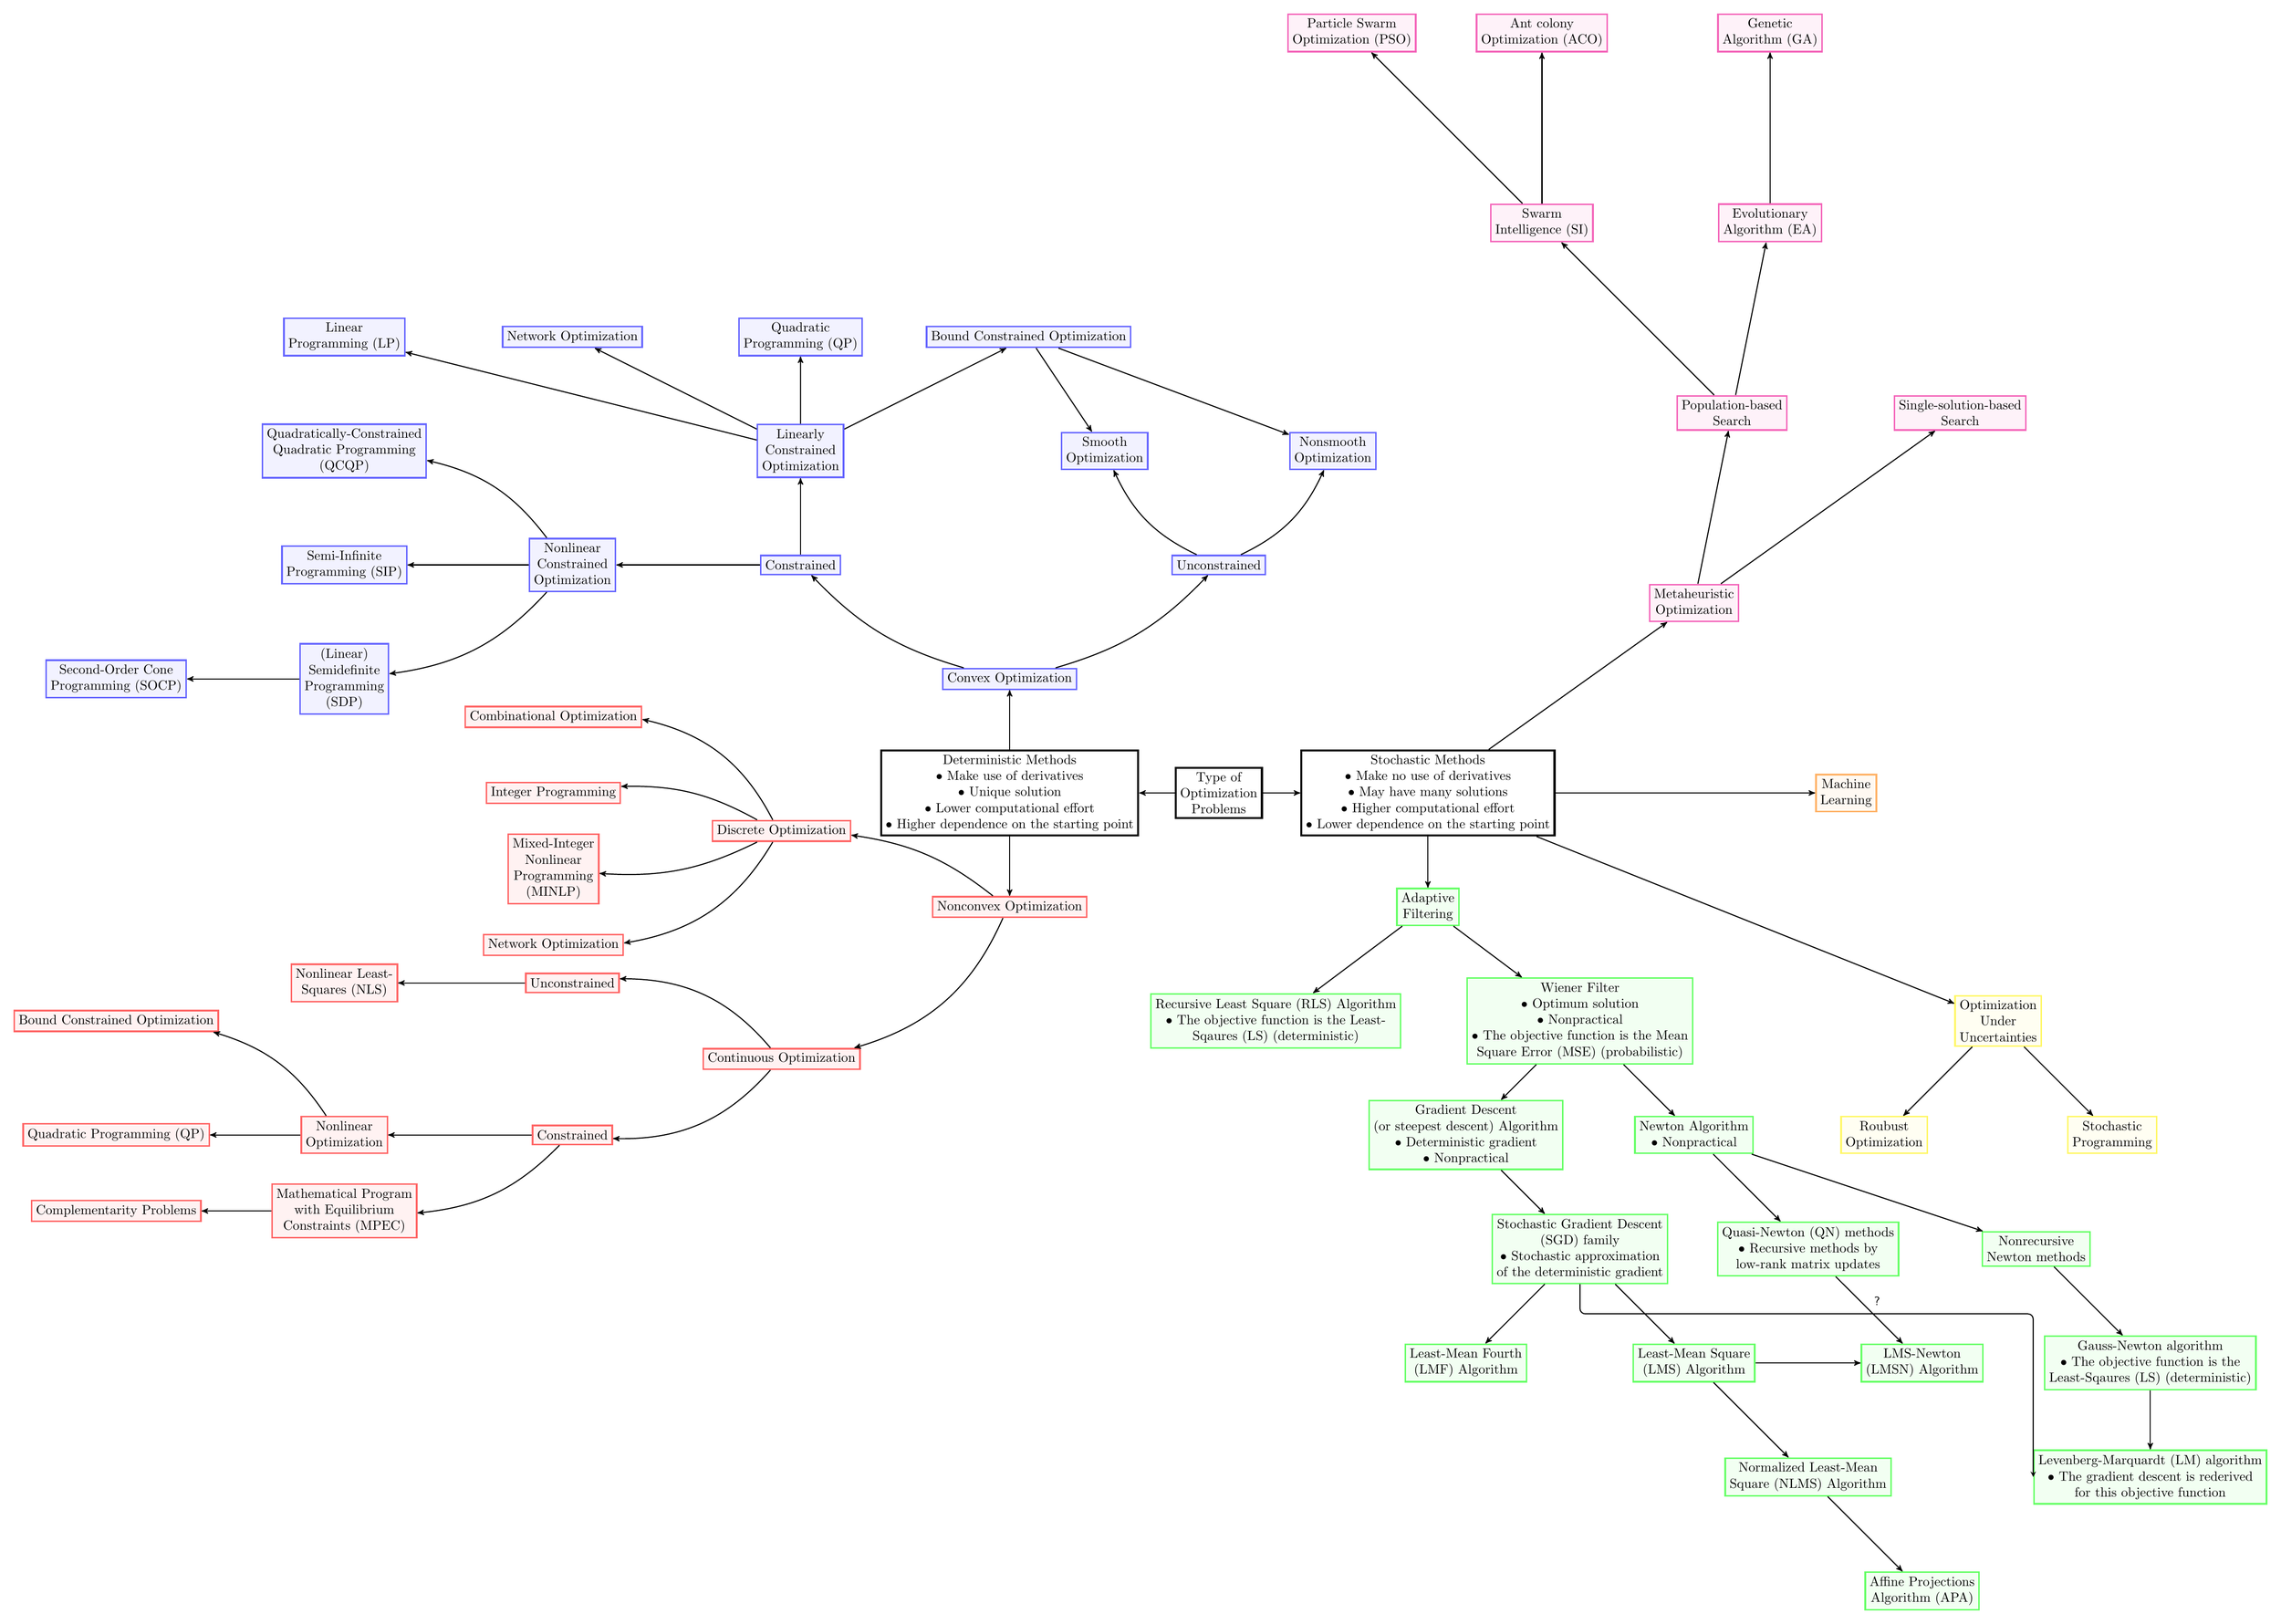
\begin{tikzpicture}[
    ->, % make tip
    >=stealth', % make the arrow's tip prettier (stealth style)
    auto,
    node distance=3cm,
    thick, % make the arrow's width thickier
    nconvex/.style={rectangle, draw=red!60, fill=red!5, very thick, minimum size=5mm},
    covex/.style={rectangle, draw=blue!60, fill=blue!5, very thick, minimum size=5mm},
    metaheuristic/.style={rectangle, draw=magenta!60, fill=magenta!5, very thick, minimum size=5mm},
    ml/.style={rectangle, draw=orange!60, fill=orange!5, very thick, minimum size=5mm},
    adapfilt/.style={rectangle, draw=green!60, fill=green!5, very thick, minimum size=5mm},
    uncertainties/.style={rectangle, draw=yellow!60, fill=yellow!5, very thick, minimum size=5mm},
    main/.style={rectangle, draw, ultra thick},
    ]
    %main Nodes
    \node[main, align=center]      (opt)  {Type of\\Optimization\\Problems};
    \node[main, align=center]      (deterministic)  [left of=opt, xshift=-2.5cm]  {Deterministic Methods\\ $\bullet$ Make use of derivatives\\ $\bullet$ Unique solution \\ $\bullet$ Lower computational effort\\ $\bullet$ Higher dependence on the starting point};
    \node[main, align=center]      (stochasticmet)  [right of=opt, xshift=2.5cm]  {Stochastic Methods\\ $\bullet$ Make no use of derivatives\\ $\bullet$ May have many solutions \\ $\bullet$ Higher computational effort \\ $\bullet$ Lower dependence on the starting point};
    
    % convex branch
    \node[covex]      (convex)          [above of=deterministic]                        {Convex Optimization};
    \node[covex]      (constrained)     [above of=convex, left of=convex, xshift=-2.5cm]    {Constrained};
    \node[covex]      (unconstrained)   [above of=convex, right of=convex, xshift=2.5cm]    {Unconstrained};
    %% constrained branch
    \node[covex, align=center]      (linconstopt)   [above of=constrained]    {Linearly\\Constrained\\Optimization};
    \node[covex, align=center]      (nonlinconstopt)   [left of=constrained, , xshift=-3cm]    {Nonlinear\\Constrained\\Optimization};

    %%% Linearly constrained optimization branch
    \node[covex, align=center]      (lp)   [left of=linconstopt, above of=linconstopt, xshift=-9cm]    {Linear\\Programming (LP)};
    \node[covex, align=center]  (network2) [right of=lp, xshift=3cm] {Network Optimization};
    \node[covex, align=center]  (qp) [right of=network2, xshift=3cm] {Quadratic\\Programming (QP)};
    \node[covex, align=center]  (boundconstopt) [right of=qp, xshift=3cm] {Bound Constrained Optimization};
    
    %% constrained branch
    \node[covex, align=center]      (smoothopt)   [above of=unconstrained, left of=unconstrained]    {Smooth\\Optimization};
    \node[covex, align=center]      (nsmoothopt)   [right of=smoothopt, xshift=3cm]    {Nonsmooth\\Optimization};
    
    %%% Nonlinear Constrained Optimization branch
    \node[covex, align=center]      (qcqp)   [left of=nonlinconstopt, above of=nonlinconstopt, xshift=-3cm]    {Quadratically-Constrained\\Quadratic Programming\\(QCQP)};
    \node[covex, align=center]      (sip)   [below of=qcqp]    {Semi-Infinite\\Programming (SIP)};
    \node[covex, align=center]      (sdp)   [below of=sip]    {(Linear)\\Semidefinite\\Programming\\(SDP)};
    %%%% Semidefinite Programming (SDP) branch
    \node[covex, align=center]      (socp)   [left of=sdp, xshift=-3cm]    {Second-Order Cone\\Programming (SOCP)};


    % nonconvex branch
    \node[nconvex]                  (nconvex)       [below of=deterministic]     {Nonconvex Optimization};
    \node[nconvex]                  (continuous)       [left of=nconvex, xshift=-3cm, yshift=-4cm]     {Continuous 
    Optimization};
    \node[nconvex] (discrete) [left of=nconvex, xshift=-3cm, yshift=2cm] {Discrete Optimization};
    %% discrete branch
    \node[nconvex]  (combinational) [left of=discrete, xshift=-3cm, yshift=3cm] {Combinational Optimization};
    \node[nconvex]  (integer) [left of=discrete, xshift=-3cm, yshift=1cm] {Integer Programming};
    \node[nconvex, align=center]  (minlp) [left of=discrete, xshift=-3cm, yshift=-1cm] {Mixed-Integer\\Nonlinear\\Programming\\(MINLP)};
    \node[nconvex, align=center]  (network) [left of=discrete, xshift=-3cm, yshift=-3cm] {Network Optimization};
    %% continuous branch
    \node[nconvex]      (cunconstrained)     [above of=continuous, left of=continuous, xshift=-2.5cm, yshift=-1cm]    {Unconstrained};
    \node[nconvex]      (cconstrained)   [below of=continuous, left of=continuous, xshift=-2.5cm, yshift=1cm]    {Constrained};
    %%% continuous branch unconstrained
    \node[nconvex, align=center]      (nls)     [left of=cunconstrained, xshift=-3cm]    {Nonlinear Least-\\Squares (NLS)};
    %%% continuous branch constrained
    \node[nconvex, align=center]      (nopt)     [left of=cconstrained, xshift=-3cm]    {Nonlinear\\Optimization};
    \node[nconvex, align=center]      (mpec)     [below of=nopt, yshift=1cm]    {Mathematical Program\\with Equilibrium\\Constraints (MPEC)};
    %%%% MPEC branch
    \node[nconvex, align=center]      (complementarity)     [left of=mpec, xshift=-3cm]    {Complementarity Problems};
    %%%% nop branch
    \node[nconvex, align=center]      (qp2)     [left of=nopt, xshift=-3cm]    {Quadratic Programming (QP)};
    \node[nconvex, align=center]      (boundconstopt2)     [left of=nopt, above of=nopt, xshift=-3cm]    {Bound Constrained Optimization};


    % underuncert branch
    \node[uncertainties, align=center]      (underuncert)   [below of=stochasticmet, right of=stochasticmet, xshift=12cm, yshift=-3cm] {Optimization\\Under\\Uncertainties};
    \node[uncertainties, align=center]      (roubust)   [below of=underuncert,left of=underuncert]                 {Roubust\\Optimization};
    \node[uncertainties, align=center]      (stochastic)   [below of=underuncert,right of=underuncert]                 {Stochastic\\Programming};

    % metaheuristic branch
    \node[metaheuristic, align=center]      (metaheuristic)   [above of=stochasticmet, right of=stochasticmet, xshift=4cm, yshift=2cm] {Metaheuristic\\Optimization};
    \node[metaheuristic, align=center]      (singlesearch)   [above of=metaheuristic, right of=metaheuristic, xshift=4cm, yshift=2cm] {Single-solution-based\\Search};
    \node[metaheuristic, align=center]      (populationsearch)   [above of=metaheuristic, left of=metaheuristic, xshift=4cm, yshift=2cm] {Population-based\\Search};
    % population search branch
    \node[metaheuristic, align=center]      (swarmintelligence)   [above of=populationsearch, left of=populationsearch, xshift=-2cm, yshift=2cm] {Swarm\\Intelligence (SI)};
    \node[metaheuristic, align=center]      (evolutionary)   [above of=populationsearch, right of=populationsearch, xshift=-2cm, yshift=2cm] {Evolutionary\\Algorithm (EA)};
    % swarm intelligence branch
    \node[metaheuristic, align=center]      (pso)   [above of=swarmintelligence, left of=swarmintelligence, xshift=-2cm, yshift=2cm] {Particle Swarm\\Optimization (PSO)};
    \node[metaheuristic, align=center]      (aco)  [right of=pso, xshift=2cm] {Ant colony\\Optimization (ACO)};
    % evolutionary branch
    \node[metaheuristic, align=center]      (ga)  [above of=evolutionary, yshift=2cm] {Genetic\\Algorithm (GA)};

    % machine learning branch
    \node[ml, align=center]      (ml)   [right of=stochasticmet, xshift=8cm] {Machine\\Learning};
    
    % adaptive filters
    \node[adapfilt, align=center]      (adapfilt)   [below of=stochasticmet] {Adaptive\\Filtering};
    \node[adapfilt, align=center]      (rls)   [below of=adapfilt, left of=adapfilt, xshift=-1cm] {Recursive Least Square (RLS) Algorithm\\$\bullet$ The objective function is the Least-\\Sqaures (LS) (deterministic)};
    \node[adapfilt, align=center]      (wiener)   [below of=adapfilt, right of=adapfilt, xshift=1cm] {Wiener Filter\\$\bullet$ Optimum solution\\$\bullet$ Nonpractical\\$\bullet$ The objective function is the Mean\\Square Error (MSE) (probabilistic)};
    \node[adapfilt, align=center]      (gradientdescent)   [below of=wiener, left of=wiener] {Gradient Descent\\(or steepest descent) Algorithm\\$\bullet$ Deterministic gradient\\$\bullet$ Nonpractical};
    \node[adapfilt, align=center]      (newton)   [below of=wiener, right of=wiener] {Newton Algorithm\\$\bullet$ Nonpractical};
    \node[adapfilt, align=center]      (sgd)   [below of=gradientdescent, right of=gradientdescent] {Stochastic Gradient Descent\\(SGD) family\\$\bullet$ Stochastic approximation \\ of the deterministic gradient};
    \node[adapfilt, align=center]      (lms)   [below of=sgd, right of=sgd] {Least-Mean Square\\(LMS) Algorithm};
    \node[adapfilt, align=center]      (lmf)   [below of=sgd, left of=sgd] {Least-Mean Fourth\\(LMF) Algorithm};
    \node[adapfilt, align=center]      (nlms)   [below of=lms, right of=lms] {Normalized Least-Mean\\Square (NLMS) Algorithm};
    \node[adapfilt, align=center]      (apa)   [below of=nlms, right of=nlms] {Affine Projections \\Algorithm (APA)};
    \node[adapfilt, align=center]      (qn)   [right of=lms, below of=newton] {Quasi-Newton (QN) methods \\ $\bullet$ Recursive methods by\\low-rank matrix updates};
    \node[adapfilt, align=center]      (nrec-newton)   [right of=qn, xshift=3cm] {Nonrecursive\\Newton methods};
    \node[adapfilt, align=center]      (lmsn)   [right of=qn, below of=qn] {LMS-Newton\\(LMSN) Algorithm};
    \node[adapfilt, align=center]      (gauss-newton)   [right of=lmsn, xshift=3cm] {Gauss-Newton algorithm\\$\bullet$ The objective function is the\\Least-Sqaures (LS) (deterministic)};
    \node[adapfilt, align=center]      (lm)   [below of=gauss-newton] {Levenberg-Marquardt (LM) algorithm\\$\bullet$ The gradient descent is rederived\\for this objective function};
    
    \path[every node/.style={font=\sffamily\small}]
    % lines from opt
    (opt) edge node [] {} (deterministic)
    (opt) edge node [] {} (stochasticmet)
    (stochasticmet) edge node [] {} (underuncert)
    (stochasticmet) edge node [] {} (ml)
    (stochasticmet) edge node [] {} (metaheuristic)
    (stochasticmet) edge node [] {} (adapfilt)
    (deterministic) edge node [] {} (nconvex)
    (deterministic) edge node [] {} (convex)
    % lines from convex
    (convex) edge[bend left=15] node [] {} (constrained)
    (convex) edge[bend right=15] node [] {} (unconstrained)
    % lines from unconstrained
    (unconstrained) edge[bend left=20] node [] {} (smoothopt)
    (unconstrained) edge[bend right=20] node [] {} (nsmoothopt)
    % lines from constrained
    (constrained) edge node [] {} (linconstopt)
    (constrained) edge node [] {} (nonlinconstopt)
    % lines from linconstopt
    (linconstopt) edge node [] {} (lp)
    (linconstopt) edge node [] {} (network2)
    (linconstopt) edge node [] {} (boundconstopt)
    (linconstopt) edge node [] {} (qp)
    % lines from boundconstopt
    (boundconstopt) edge node [] {} (smoothopt)
    (boundconstopt) edge node [] {} (nsmoothopt)
    % lines from nonlinconstopt
    (nonlinconstopt) edge[bend right=20] node [] {} (qcqp)
    (nonlinconstopt) edge[] node [] {} (sip)
    (nonlinconstopt) edge[bend left=20] node [] {} (sdp)
    % lines from sdp
    (sdp) edge[] node [] {} (socp)
    % lines from underuncert
    (underuncert) edge node [] {} (roubust)
    (underuncert) edge node [] {} (stochastic)
    % lines from nconvex
    (nconvex) edge[bend left=25] node [] {} (continuous)
    
    (nconvex) edge[bend right=15] node [] {} (discrete)
    % lines from discrete
    (discrete) edge[bend right=25] node [] {} (combinational)
    (discrete) edge[right, bend right=15] node [] {} (integer)
    (discrete) edge[right, bend left=15] node [] {} (minlp)
    (discrete) edge[right, bend left=25] node [] {} (network)
    % lines from continuous
    (continuous) edge[bend right=25] node [] {} (cunconstrained)
    (continuous) edge[bend left=25] node [] {} (cconstrained)
    % lines from cunconstrained
    (cunconstrained) edge[] node [] {} (nls)
    % lines from cconstrained
    (cconstrained) edge[] node [] {} (nopt)
    (cconstrained) edge[bend left=20] node [] {} (mpec)
    % lines from mpec
    (mpec) edge[] node [] {} (complementarity)
    % lines from nopt
    (nopt) edge[] node [] {} (qp2)
    (nopt) edge[bend right=20] node [] {} (boundconstopt2)
    % lines from adaptive filters
    (adapfilt) edge node [] {} (wiener)
    (adapfilt) edge node [] {} (rls)
    (wiener) edge node [] {} (gradientdescent)
    (wiener) edge node [] {} (newton)
    (gradientdescent) edge node [] {} (sgd)
    (sgd) edge node [] {} (lms)
    (sgd) edge node [] {} (lmf)
    (lms) edge node [] {} (nlms)
    (nlms) edge node [] {} (apa)
    (newton) edge node [] {} (qn)
    (newton) edge node [] {} (nrec-newton)
    (nrec-newton) edge node [] {} (gauss-newton)
    (gauss-newton) edge node [] {} (lm)
    % (gradientdescent) edge[bend left=20] node [] {} (lm)
    (qn) edge node [] {?} (lmsn)
    (lms) edge node [] {} (lmsn)
    % lines from metaheuristics
    (metaheuristic) edge node [] {} (singlesearch)
    (metaheuristic) edge node [] {} (populationsearch)
    % lines from population-based
    (populationsearch) edge node [] {} (swarmintelligence)
    (populationsearch) edge node [] {} (evolutionary)
    % lines from swarm intelligence
    (swarmintelligence) edge node [] {} (pso)
    (swarmintelligence) edge node [] {} (aco)
    % lines from evolutionary algoruthms
    (evolutionary) edge node [] {} (ga);

    \tikzstyle{arrow} = [thick,->,>=stealth]
    \draw[rounded corners, arrow]
    (sgd.south) |-
    ($ (sgd.south)!.5!(lmsn.north) $) -|
    ($(lm.west)$);

\end{tikzpicture}
\end{document}